\documentclass[journal,twoside]{IEEEtran}
\usepackage[T1]{fontenc}
\usepackage{microtype}
\DisableLigatures[<]{encoding = T1}
\DisableLigatures[>]{encoding = T1}
\usepackage{graphicx}
\usepackage{booktabs}
\usepackage{multicol,multirow}
\usepackage{newtxmath}
\usepackage{mathtools}
\usepackage{bm}
\usepackage[caption=false,font=footnotesize,subrefformat=parens]{subfig}
\usepackage{lipsum}
\usepackage{tabularx}
\usepackage[dvipsnames,table]{xcolor}
\usepackage{my-tikz}
\usepackage{colortbl}
\usepackage{scalerel}
\usepackage{threeparttable}
\usepackage{algorithm}
\usepackage[italicComments=false,commentColor=darkgray,noEnd=true]{algpseudocodex}
\usepackage{upgreek}
\usepackage{calc}
\usepackage[noadjust]{cite}
\usepackage{circuitikz}
\usepackage{siunitx}
\usepackage{minted}
\usepackage[colorlinks,urlcolor=black,linkcolor=blue,citecolor=blue]{hyperref}

\usetikzlibrary{svg.path,shapes.symbols,shapes.misc}
\usepgfplotslibrary{fillbetween}
\definecolor{orcidlogocol}{HTML}{A6CE39}
\tikzset{
  orcidlogo/.pic={
    \fill[orcidlogocol] svg{M256,128c0,70.7-57.3,128-128,128C57.3,256,0,198.7,0,128C0,57.3,57.3,0,128,0C198.7,0,256,57.3,256,128z};
    \fill[white] svg{M86.3,186.2H70.9V79.1h15.4v48.4V186.2z}
                 svg{M108.9,79.1h41.6c39.6,0,57,28.3,57,53.6c0,27.5-21.5,53.6-56.8,53.6h-41.8V79.1z M124.3,172.4h24.5c34.9,0,42.9-26.5,42.9-39.7c0-21.5-13.7-39.7-43.7-39.7h-23.7V172.4z}
                 svg{M88.7,56.8c0,5.5-4.5,10.1-10.1,10.1c-5.6,0-10.1-4.6-10.1-10.1c0-5.6,4.5-10.1,10.1-10.1C84.2,46.7,88.7,51.3,88.7,56.8z};
  }
}

\newcommand\orcidicon[1]{\href{https://orcid.org/#1}{\mbox{\scalerel*{
  
\begin{tikzpicture}[yscale=-1,transform shape]
    \pic{orcidlogo};
  \end{tikzpicture}
}{|}}}}

% \makesavenoteenv{tabular}
\interdisplaylinepenalty=2500
\aboverulesep = 0mm \belowrulesep = 0mm
\newcolumntype{Y}{>{\centering\arraybackslash}X}
\newcolumntype{M}[1]{>{\centering\arraybackslash}m{#1}} % centered m
\newcommand{\tabvertspace}{\specialrule{0em}{0.08em}{.08em}}
\renewcommand\tabularxcolumn[1]{m{#1}}% for vertical centering text in X column

\definecolor{doicolor}{RGB}{2, 48, 129}

\DeclareMathOperator*{\argmax}{\arg\max}
\DeclareMathOperator*{\argmin}{\arg\min}
\DeclareMathOperator*{\argmint}{\widetilde{\arg\min}}
\DeclareMathOperator*{\uargmin}{\mathrm{u}\arg\min}

\setlength{\fboxsep}{0pt}
\setminted{
  , frame = lines
  , fontsize = \scriptsize
  , bgcolor = gray!3
  , framesep = 2.5pt
}

\markboth{Southeast University Software-Defined Radio Experiment Course, January 2024}{W. Zhao: Dual-Mode PSK Transceiver on SDR With FPGA}
\IEEEpubid{
  \begin{tabular}[t]{c}
    \copyright{} 2024 Wuqiong Zhao.
    This work is licensed under a Creative Commons Attribution-ShareAlike 4.0 License.\\
    For more information, see \url{https://creativecommons.org/licenses/by-sa/4.0/}.
  \end{tabular}
}

\hypersetup{
  , pdftitle    = {Dual-Mode {PSK} Transceiver on {SDR} With {FPGA}}
  , pdfauthor   = {Wuqiong Zhao}
  , pdfsubject  = {Southeast University Software-Defined Radio Experiment Course}
  , pdfkeywords = {Phase-shift keying (PSK), software-defined radio (SDR), transceiver design, modulation, demodulation, field programmable gate array (FPGA).}
}

\begin{document}

  \title{Dual-Mode PSK Transceiver on SDR With FPGA}

  \author{%
    Wuqiong~Zhao{\hspace{.1em}\textsuperscript{\orcidicon{0000-0002-9550-7423}}},~\IEEEmembership{Student Member, IEEE}
    \thanks{Date of publication 7 January 2024; date of current version 7 January 2024.
      The author would like to thank Lecturer Dan Yang for the guidance and help in the course of the experiment.
      The author would also like to thank AI tools including GitHub Copilot and Claude.AI for their help in preparing this paper.}
    \thanks{Wuqiong Zhao is with Southeast University, Nanjing 211189, China. (e-mail: wqzhao@seu.edu.cn, website: \url{https://wqzhao.org}).}
    \thanks{Online URL: \url{https://go.wqzhao.org/sdr-psk-fpga}}
    % \vspace{-1mm}
  }

  \IEEEspecialpapernotice{(This is a draft version and has not been completed yet.)}

  \maketitle

  \begin{abstract}
    In this experiment, we implement a dual-mode PSK transceiver on SDR with FPGA,
    supporting both BPSK and QPSK.
    Moreover, the transceiver is designed to be able to switch between the two modes by introducing packet-based communication,
    where modulation information can be extracted from the packet header.
  \end{abstract}
  \begin{IEEEkeywords}
    Phase-shift keying (PSK), software-defined radio (SDR), transceiver design, modulation, demodulation, field programmable gate array (FPGA).
  \end{IEEEkeywords}

  \section{Introduction}

    \IEEEPARstart{S}{oftware-defined} radio (SDR) is interesting, like application in millimeter wave \cite{zhao2020m}.
    FPGA is also interesting!

    Instead of employing high-level synthesis (HLS) \cite{zhao2023flexible},
    we directly implement the transceiver on FPGA using hardware description language (HDL) Verilog,
    for a better control of the underlying hardware.

    The design source (Vivado project) and this paper (in \LaTeX) are open source \cite{github_repo}.
    

  \section{System Overview}

    \subsection{Software-Defined Radio}

      eNodeX

    \subsection{Transceiver Design}

      The current transmitter and receiver are implemented on the same FPGA,
      but can be readily extended to different FPGAs with small frequency offsets.
      The system overview is shown in Fig.~\ref{fig:system_overview}.
      \begin{figure}[htbp]
        \centering
        \begin{tikzpicture}[
  , thick
  , n/.style = {
    , draw
    , fill = myblued!15
    , align = center
  }
  , font = \small\sffamily
]
  \node [n] {RF Data\\Converter};
\end{tikzpicture}%

        \caption{Transceiver system overview.}
        \label{fig:system_overview}
      \end{figure}

      \textbf{Clock Generator}.
      All reset signals are generated using Processor System Reset Modules \cite{xilinx:pg164},
      which can provide synchronized power-up reset signals.

      \textbf{RF Data Converter}.
      This block is contains analog-to-digital converter (ADC) and digital-to-analog converter (DAC),
      enabled by a vendored AD9361 module.

      \textbf{Tx Signal Generator}.

      \textbf{Rx Processor}.
      This block is responsible to process the received signal,
      including demodulation and data extraction from a packet.
      It is the most complicated block in the system.

      \textbf{System ILA}.
      The system integrated logic analyzer (system ILA) \cite{xilinx:pg261} is used to observe the internal signals.

      \textbf{Constant Configurations}.
      Several parameters can be configured in this block.
      Most importantly, the mode control constants (\texttt{MODE\_CTRL}) are shown in Table~\ref{tab:mode_ctrl}.
      \begin{table}[htbp]
        \caption{Mode Control Constants}
        \label{tab:mode_ctrl}
        \renewcommand{\arraystretch}{1.2}
        \rowcolors{1}{white}{gray!15}
        \begin{tabularx}{\linewidth}{cYYYc}
          \toprule\tabvertspace
          \textbf{Mode} & \textbf{Localparam} & \textbf{Value} & \textbf{\ttfamily is\_bpsk} & \textbf{Packet} \\
          \tabvertspace\midrule
            BPSK & \texttt{MODE\_BPSK} & \texttt{4\textquotesingle b0001} (1) & \texttt{1\textquotesingle b1} & No \\
            QPSK & \texttt{MODE\_QPSK} & \texttt{4\textquotesingle b0010} (2) & \texttt{1\textquotesingle b0} & No \\
            Mixed & \texttt{MODE\_MIX~~} & \texttt{4\textquotesingle b0100} (4) & variable & Yes \\
          \bottomrule
        \end{tabularx}
      \end{table}

    \subsection{BPSK/QPSK Modulation}

      The BPSK and QPSK modulation constellation graphs used in our system are shown in Fig.~\ref{fig:constellation}.
      Different from the traditional setting, out adopted BPSK constellation in Fig.~\subref*{subfig:constellation_BPSK}
      is a combination of I and Q components.
      This is to make sure the phases used in BPSK are among those in QPSK,
      to ensure a smooth transition between the two modes,
      especially because the header field is always modulated in BPSK.
      \begin{figure}[htbp]
        \subfloat[BPSK.\label{subfig:constellation_BPSK}]{\begin{tikzpicture}[
  , thick
  , axis/.style = {
    , -latex
  }
  , n/.style = {
    , circle
    , fill = myblued
    , inner sep = 0pt
    , minimum size = 4pt
  }
  , l/.style = {
    , dotted
  }
  , ll/.style = {
    , dashed
    , myred
    , shorten < = -8pt
    , shorten > = -8pt
  }
  , outer sep = 0
  , inner sep = 2pt
]
  \draw [axis] (-1.5, 0) -- (1.5, 0) [right] node {$I\,(\cos)$};
  \draw [axis] (0, -1.5) -- (0, 1.5) [above] node {$Q\,(\sin)$};
  \draw [ll] (-1, 1) -- (1, -1);
  \draw [l] (0, 1) -- (1, 1);
  \draw [l] (0, -1) -- (-1, -1);
  \draw [l] (1, 0) -- (1, 1);
  \draw [l] (-1, 0) -- (-1, -1);
  \node [n, label={right:\ttfamily\bfseries0}] at (1, 1) {};
  \node [n, label={left:\ttfamily\bfseries1}] at (-1, -1) {};
\end{tikzpicture}%
}\hfill%
        \subfloat[QPSK.\label{subfig:constellation_QPSK}]{\begin{tikzpicture}[
  , thick
  , axis/.style = {
    , -latex
  }
  , n/.style = {
    , circle
    , fill = myblued
    , inner sep = 0pt
    , minimum size = 4pt
  }
  , l/.style = {
    , dotted
  }
  , ll/.style = {
    , dashed
    , myred
    , shorten < = -8pt
    , shorten > = -8pt
  }
  , outer sep = 0
  , inner sep = 2pt
]
  \draw [axis] (-1.5, 0) -- (1.5, 0) [right] node {$I\,(\cos)$};
  \draw [axis] (0, -1.5) -- (0, 1.5) [above] node {$Q\,(\sin)$};
  \draw [l] (-1, 1) -- (1, 1);
  \draw [l] (1, -1) -- (-1, -1);
  \draw [l] (1, -1) -- (1, 1);
  \draw [l] (-1, 1) -- (-1, -1);
  \node [n, label={right:\ttfamily\bfseries00}] at (1, 1) {};
  \node [n, label={below:\ttfamily\bfseries01}] at (1, -1) {};
  \node [n, label={left:\ttfamily\bfseries11}] at (-1, -1) {};
  \node [n, label={above:\ttfamily\bfseries10}] at (-1, 1) {};
\end{tikzpicture}%
}
        \caption{BPSK/QPSK modulation constellation used in our system.}
        \label{fig:constellation}
      \end{figure}

    \IEEEpubidadjcol
    \section{Transmitter}

    \subsection{Carrier NCO}

      The carrier frequency is generated by a numerically controlled oscillator (NCO).
      In Vivado, we use the Direct Digital Synthesis (DDS) Compiler IP core to generate the NCO.

  \subsection{PSK Modulation}

    \subsubsection{Pseudo-random Noise (PN) Generator}

      In this experiment, the transmitted signal are pseudo-random noise (PN) sequences.
      Typically, we implement the PN generator with $N=4$ and $N=5$. % mention the structure here
      The Verilog code for the module \texttt{PN\_Gen} is shown below.
      \begin{minted}[highlightlines={11,18}]{verilog}
module PN_Gen # (parameter N = 5) (
  input      clk,
  output reg pn
);
  reg [N-1:0] PN_buf = 1; wire rst;
  generate
  if (N == 5)
    always @ (posedge clk)
      if (rst) begin PN_buf <= 5'd1; pn <= 0; end
      else begin
        PN_buf <= { PN_buf[3:0], PN_buf[4] ^ PN_buf[2] };
        pn <= PN_buf[4];
      end
  else if (N == 4)
    always @ (posedge clk)
      if (rst) begin PN_buf <= 4'd1; pn <= 0; end
      else begin
        PN_buf <= { PN_buf[2:0], PN_buf[3] + PN_buf[2] };
        pn <= PN_buf[3];
      end
  else ; // NOT implemented yet!
  endgenerate
  assign rst = !(|PN_buf);  // reset when PN_buf is all 0
endmodule
      \end{minted}

    \subsubsection{Modulation With I and Q Streams}

      The modulation is performed by multiplying selecting the appropriate carrier phase
      according to the input bits and the constellation.
      Note the Q component always has a phase $90^\circ$ ahead of the I component.

  \section{Receiver}

    \subsection{Overview}

      The receiver performs carrier synchronization, symbol synchronization and PSK detection first,
      without considering the packet structure.
      The depacketizer and the packet extraction is based on the synchronized bit stream after PSK detection.

    \subsection{Carrier Synchronization Using Costas Loop}

      A Costas loop \cite{simon1977optimum} is used for carrier synchronization.
      The basic idea of a Costas loop is to provide an error (carrier phase offset) feedback.
      The negative feedback is used to lock the carrier phase to the PSK signal.
      The generation of the error feedback is specific to different modulation schemes,
      as well as their constellation graphs.

      The proposed dual-mode Costas loop is shown in Fig.~\ref{fig:costas_loop},
      which can be switched between BPSK and QPSK via a control signal \texttt{is\_bpsk}.
      The two multipliers directly following the PSK stream input are phase detectors,
      whose low-frequency components represent the baseband signal.
      Therefore, the baseband I and Q signal can be extracted after passing through a low-pass filter (LPF).
      Thus, it is ready to map the obtained I/Q signal to the constellation graph,
      and generate the error signal when comparing with the designed one.
      \begin{figure}[htbp]
        \centering
        \begin{tikzpicture}[
  , thick
  , font = \small\sffamily
  , node distance = 8mm and 5mm
  , 1bit/.style = {
    , semithick
  }
  , font xs/.style = {
    , font = \notsotiny\sffamily
  }
  , n/.style = {
    , draw
    , minimum height = 5mm
    , fill = #1!15
  }
  , n/.default = myblued
  , LPF/.style = {
    , n = myyellow
    , minimum width = 6mm
  }
  , arr/.style = {
    , -latex
  }
  , arr r/.style = {
    , latex-
  }
  , port/.style = {
    , n = gray
    , signal
    , signal to = east
    , minimum height = 2mm
  }
  , port label/.style = {
    , font xs
    , align = center
    , below = 1mm
  }
  , mul add base/.style = {
    , draw = black
    , circle
    , minimum width = 3mm
    , fill = none
  }
  , add/.style = {
    , mul add base
    , append after command = {
      \pgfextra
        \draw [-, black] (\tikzlastnode.north) -- (\tikzlastnode.south);
        \draw [-, black] (\tikzlastnode.east)  -- (\tikzlastnode.west);
      \endpgfextra
    }
  }
  , sub/.style = {
    , mul add base
    , append after command = {
      \pgfextra
        \draw [-, black] (\tikzlastnode.north) -- (\tikzlastnode.south);
        \draw [-, black] (\tikzlastnode.east)  -- (\tikzlastnode.west);
        \node [above left = 0mm and 0mm of \tikzlastnode.north, inner sep = 0] {\notsotiny\resizebox*{\widthof{+}}{\heightof{-}}{-}};
        \node [above right = 0mm and 0mm of \tikzlastnode.east, inner sep = 0] {\notsotiny+};
      \endpgfextra
    }
  }
  , mul/.style = {
    , mul add base
    , append after command = {
      \pgfextra
        \draw [-, black] (\tikzlastnode.north west) -- (\tikzlastnode.south east);
        \draw [-, black] (\tikzlastnode.north east) -- (\tikzlastnode.south west);
      \endpgfextra
    }
  }
  , null node/.style = {
    , inner sep = 0
    , outer sep = 0
    , minimum width = 0
    , 
  }
  , joint/.style = {
    , circle
    , minimum height = 0.8mm
    , inner sep = 0
    , fill = #1
    , draw = #1
  }
  , joint/.default = black
  , mux/.style = {
    , n = mygreen
    , trapezium
    , trapezium angle = 60
    , shape border rotate = 90
    , minimum height = 3.8mm
    , anchor = south
  }
]
  \node (nco) [n] {NCO};
  \node (loop-filter) [LPF, right = of nco] {};

  \node (lpf-I) [LPF, above = of loop-filter] {};
  \node (lpf-Q) [LPF, below = of loop-filter] {};

  \node (mul-I) [mul, xshift = -7mm] at (nco |- lpf-I) {};
  \node (mul-Q) [mul, xshift = -7mm] at (nco |- lpf-Q) {};

  \node (in-j) [joint, left = 8mm of nco] {};
  
  \draw [arr] (loop-filter) -- (nco);
  \draw [arr] ([yshift = +1mm]nco.west) -| (mul-I) node [midway, right, yshift = +7mm] {$\cos$};
  \draw [arr] ([yshift = -1mm]nco.west) -| (mul-Q) node [midway, right, yshift = -7mm] {$\sin$};

  % input port
  \draw (in-j) -- ++ (-6mm, 0) node [port] {}
                               node (in-psk) [port label] {PSK\\strm.};

  % mux
  \draw [arr r] (loop-filter.east) -- ++ (5mm, 0) node (mux) [mux, right] {}
                                                  node [font xs, above right = .5mm and 1.2mm, inner sep = 0] {0}
                                                  node [font xs, below right = .5mm and 1.2mm, inner sep = 0] {1};
  \draw [1bit, shorten < = -.1mm] (mux.north)
    to [jump, jump pos = .595, |u-, jump swap] ([yshift = 5mm] in-psk |- mul-I.north) node [port] {}
                                                                                      node [port label] {is\_bpsk};

  % error output
  \node [sub, right = of mux.east, yshift = +2.2mm] (sub-QPSK) {};
  \draw [arr] (sub-QPSK) -- (sub-QPSK.west -| mux.east);
  \node [mul, right = of mux.east, yshift = -2.2mm] (mul-BPSK) {};
  \draw [arr] (mul-BPSK) -- (mul-BPSK.west -| mux.east);

  % error detector
  \node (err-detect-ctrl) [n = myred, align = center, anchor = west] at ([xshift = 10mm] mul-BPSK.east |- loop-filter.east) {Error\\Detector\\Control};
  \draw (sub-QPSK) -- (sub-QPSK -| err-detect-ctrl.west) node [above left, font xs, inner sep = .5mm, align = center] {\hphantom{Q}\\I};
  \draw (mul-BPSK) -- (mul-BPSK -| err-detect-ctrl.west) node [above left, font xs, inner sep = .5mm] {Q};
  \draw ([xshift = -3.5mm] sub-QPSK-| err-detect-ctrl.west) node [joint] {} to[jump, jump pos = .55] ++ (0, -8mm) -| (mul-BPSK);
  \draw ([xshift = -6.5mm] mul-BPSK-| err-detect-ctrl.west) node [joint] {} to[jump, jump pos = .55, jump swap] ++ (0, +8mm) -| (sub-QPSK);
  \node (err-detect) [fit = (err-detect-ctrl) (mux), draw, dashed, myred] {};
  \node [myred, anchor = north west, inner xsep = 0] at (err-detect.south west) {Error Detector};

  % loop filter tooltip
  \draw [thin, shorten < = .5mm] (loop-filter.south west) -- ++ (-2mm, -2mm)
                                                          -- ++ (-2mm, 0) node [left, font xs, inner sep = .5mm] {Loop Filter};
  \foreach \x in {I, Q} {
    \draw [arr] (mul-\x) -- (lpf-\x);
    \draw [arr] (in-j) |- (mul-\x);
    \draw [arr] (lpf-\x) -| (err-detect-ctrl) node (out-\x) [midway, joint] {};
    \draw (out-\x) -- ++ (5mm, 0) node [port, right, label={right:\x}] {};
  }
  
  % LPF: draw symbol and add label
  \foreach \x in {loop-filter, lpf-I, lpf-Q} {
    \draw ([xshift = -2.2mm, yshift = 1.5mm]\x.center) -- ++ (1.7mm, 0)
                                                       -- ++ (1mm, -3mm)
                                                       -- ++ (1.7mm, 0);
    \node [below = .5mm of \x, font xs, inner ysep = 0] {LPF};
  }
\end{tikzpicture}%

        \caption{Costas loop for carrier synchronization with BPSK/QPSK support.}
        \label{fig:costas_loop}
      \end{figure}

      The error feedback for BPSK is defined as
      \begin{equation}
        e_{\text{BPSK}}=(I+Q)\times(I-Q),
      \end{equation}
      and the error feedback for QPSK is defined as
      \begin{equation}
        e_{\text{QPSK}}=I\cdot\mathrm{sgn}(Q)-Q\cdot\mathrm{sgn}(I).
      \end{equation}

      For stability, the loop filter as an LPF is added before the error is fed back to the NCO.     
      The NCO implemented with DDS has the phase defined as
      \begin{equation}
        \begin{aligned}
          \phi[n]&=\phi[n-1]+\Delta\phi[n]\\
          &=\phi[n-1]+(f_0+k\cdot f_{\text{feedback}}),
        \end{aligned}
      \end{equation}
      where $\phi[n]$ is the phase increment at time $n$,
      $f_0$ is the free running clock (\qty{4.096}{MHz} in our design),
      and $k$ is the feedback coefficient.
      The core Verilog implementation of the Error Detector Control is given below,
      which shows that for QPSK, the feedback value is arithmetically right shifted by 6 bits
      to match the scale of that in BPSK.
      \begin{minted}[]{verilog}
if (is_bpsk) begin // BPSK
  out_I_tdata <= in_I_tvalid ? in_I_tdata + in_Q_tdata : 0;
  out_Q_tdata <= in_Q_tvalid ? in_I_tdata - in_Q_tdata : 0;
end
else begin // QPSK
  out_I_tdata <= in_I_tvalid ? (in_Q_tdata[WIDTH-1] ?
    -in_I_tdata : in_I_tdata) >>> 6 : 0;
  out_Q_tdata <= in_Q_tvalid ? (in_I_tdata[WIDTH-1] ?
    -in_Q_tdata : in_Q_tdata) >>> 6 : 0;
end
      \end{minted}
      
      In the Costas loop,
      the feedback coefficient $k$ is an important coefficient to finetune according to the system.
      This parameter is reflected as \texttt{FEEDBACK\_SHIFT}, and $k\triangleq2^{-\text{\texttt{FEEDBACK\_SHIFT}}}$.
      The convergence of the Costas loop under different carrier frequency offset (CFO) is discussed in Section~\ref{subsec:costas_convergence}.

    \subsection{Symbol Synchronization Using Gardner Loop}

      A Gardner loop \cite{gardner1986bpsk} is used to achieve symbol (timing) synchronization.
      The structure of a Gardner loop is shown in Fig.~\ref{fig:gardner_loop}.
      The loop itself is not directly shown in the figure,
      \begin{figure}[htbp]
        \begin{tikzpicture}[
  , thick
  , font = \small\sffamily
  , node distance = 8mm and 5mm
  , 1bit/.style = {
    , semithick
  }
  , font xs/.style = {
    , font = \notsotiny\sffamily
  }
  , n/.style = {
    , draw
    , minimum height = 5mm
    , fill = #1!15
  }
  , n/.default = myblued
  , IFIR/.style = {
    , n = myyellow
    , minimum width = 6mm
  }
  , arr/.style = {
    , -latex
  }
  , arr r/.style = {
    , latex-
  }
  , port/.style = {
    , n = gray
    , signal
    , signal to = east
    , minimum height = 2mm
  }
  , port label/.style = {
    , font xs
    , align = center
    , below = 1mm
  }
  , mul add base/.style = {
    , draw = black
    , circle
    , minimum width = 3mm
    , fill = none
  }
  , add/.style = {
    , mul add base
    , append after command = {
      \pgfextra
        \draw [-, black] (\tikzlastnode.north) -- (\tikzlastnode.south);
        \draw [-, black] (\tikzlastnode.east)  -- (\tikzlastnode.west);
      \endpgfextra
    }
  }
  , sub/.style = {
    , mul add base
    , append after command = {
      \pgfextra
        \draw [-, black] (\tikzlastnode.north) -- (\tikzlastnode.south);
        \draw [-, black] (\tikzlastnode.east)  -- (\tikzlastnode.west);
        \if#11\relax
          \node [above left = 0mm and 0mm of \tikzlastnode.north, inner sep = 0] {\notsotiny+};
        \else
          \node [below left = 0mm and 0mm of \tikzlastnode.south, inner sep = 0] {\notsotiny+};
        \fi
        \node [above left = 0mm and 0mm of \tikzlastnode.west, inner sep = 0] {\notsotiny\resizebox*{\widthof{+}}{\heightof{-}}{-}};
      \endpgfextra
    }
  }
  , sub/.default = 0
  , mul/.style = {
    , mul add base
    , append after command = {
      \pgfextra
        \draw [-, black] (\tikzlastnode.north west) -- (\tikzlastnode.south east);
        \draw [-, black] (\tikzlastnode.north east) -- (\tikzlastnode.south west);
      \endpgfextra
    }
  }
  , null node/.style = {
    , inner sep = 0
    , outer sep = 0
    , minimum width = 0
    , 
  }
  , joint/.style = {
    , circle
    , minimum height = 0.8mm
    , inner sep = 0
    , fill = #1
    , draw = #1
  }
  , joint/.default = black
  , mux/.style = {
    , n = mygreen
    , trapezium
    , trapezium angle = 60
    , shape border rotate = 90
    , minimum height = 3.8mm
    , anchor = south
  }
]
  \node (ifir-I) [IFIR] {\smash{\raisebox{.2mm}{$\uparrow$}2}\vphantom{2}};
  \node (ifir-Q) [IFIR, below = of ifir-I] {\smash{\raisebox{.2mm}{$\uparrow$}2}\vphantom{2}};

  \foreach \x in {I, Q} {
    \draw (ifir-\x.west) -- ++ (-3mm, 0) node [port, left = -.5mm, label={left:\x}] (in-\x) {};
    \node [below = .5mm of ifir-\x, font xs, inner ysep = 0] {IFIR};
    \draw [arr] (ifir-\x.east) -- ++ (7mm, 0) node (D1-\x) [n, right] {16D};
    \draw [arr] (D1-\x.east) -- ++ (5mm, 0) node (D2-\x) [n, right] {16D};
    \draw [arr] (D2-\x.east) -- ++ (3mm, 0) node (sub-\x) [sub = \if\x I1\else0\fi, right] {};
    \draw [arr] (sub-\x.east) -- ++ (1.5mm, 0) node (mul-\x) [mul, right] {};
    \draw ([xshift = 3mm]ifir-\x.east) node (joint-\x) [joint] {} node [\if\x Ibelow\else above\fi, scale = .6, xshift = 1.5mm] {$y_\x(r)$} -- ++ (0, \if\x I+\else-\fi5mm) -| (sub-\x.north) {} node (y-\x) [joint, midway] {};
    \draw ([xshift = 1.5mm]D1-\x.east) node [joint] {} -- ++ (0, \if\x I-\else+\fi5mm) -| (mul-\x.\if\x Isouth\else north\fi) {} node [midway, scale = .6, \if\x Iabove left\else below left\fi, inner ysep = .5mm] {$y_\x(r-\tfrac12)$};
  }
  \node (add) [add, right = .5mm of $(mul-I.east)!.5!(mul-Q.east)$] {};
  \draw [arr] (add.east) -- ++ (3mm, 0) node [n = myred, align = center, right] (t) {Timing\\Correct.};
  \foreach \x in {I, Q} {
    \draw [arr] (mul-\x) -| (add);
    \draw [arr] (y-\x) -| (t);
  }
  \draw ([yshift = +2mm]t.east) -- ++ (3mm, 0) node (out-I) [port, right, label = {above:\scriptsize I\_1M}] {};
  \draw ([yshift = -2mm]t.east) -- ++ (3mm, 0) node (out-Q) [port, right, label = {below:\scriptsize Q\_1M}] {};
  \draw ([xshift = 4mm]t.south) |- ([yshift = -5mm] out-Q |- t.south) node [port, label = {below:\scriptsize clk\_1M}] {};

  \node (err-detect) [draw, dashed, mygreen, fit = (add)(joint-I)(joint-Q), inner ysep = 6mm] {};
  \node [mygreen, anchor = north, inner ysep = 0, yshift = -.5mm] at (err-detect.south) {Timing Error Detector};
\end{tikzpicture}%

        \caption{Structure of a Gardner loop for symbol timing synchronization.}
        \label{fig:gardner_loop}
      \end{figure}

      To reduce implementation complexity, we use the sign of strobe values as mentioned in \cite{gardner1986bpsk}.
      The total symbol timing error considering I and Q components is
      \begin{equation}
        \begin{aligned}
          u_t(r)&=y_I(r-\tfrac12)\left[\mathrm{sgn}\left(y_I(r)\right)-\mathrm{sgn}\left(y_I(r-1)\right)\right] \\
          &\quad{}+y_Q(r-\tfrac12)\left[\mathrm{sgn}\left(y_Q(r)\right)-\mathrm{sgn}\left(y_Q(r-1)\right)\right],
        \end{aligned}
      \end{equation}
      where $r$ has a symbol frequency of \qty{1.024}{MHz}.
      For better timing performance, we linearly interpolate the \qty{16.385}{MHz} input I/Q data to \qty{32.768}{MHz}.
      Therefore, $y_I(r-1)$ and $y_Q(r-1)$ are delayed by 32 clocks.
      In FPGA implementation, for each I/Q stream, two shift registers of depth 16 are used.
      Notably, since we adopt the BPSK constellation in Fig.~\subref*{subfig:constellation_BPSK},
      the symbol timing error depends on both I and Q components, the same as QPSK.

  \section{Packet-Based Communication}

    \subsection{Frame Structure}\label{subsec:frame_structure}

      The frame structure is shown in Fig.~\ref{fig:frame_structure}.
      \begin{figure}[htbp]
        \centering
        \begin{tikzpicture}[
  , thick
  , inner sep = 0
  , outer sep = 0
  , n/.style = {
    , draw
    , fill = #1!15
    , minimum height = 12pt
  }
  , node distance = -.5\pgflinewidth
  , font = \small\sffamily
  , dl/.style = {
    , semithick
    , densely dotted
  }
]
  \node [n = myblued, minimum width = 18pt] (TRN-1) {$\mathbf{D}$};
  \node [n = myblued, minimum width = 18pt, right = of TRN-1] (TRN-2) {$\mathbf{D}$};
  \node [n = myblued, minimum width = 18pt, right = of TRN-2] (TRN-3) {$\dots$};
  \node [n = myblued, minimum width = 18pt, right = of TRN-3] (TRN-4) {$\mathbf{D}$};
  \node [n = mygreen, minimum width = 18pt, right = of TRN-4] (TRN-5) {$\overline{\mathbf{D}}$};
  \node [n = myred, minimum width = 36pt, right = of TRN-5] (HDR) {HDR};
  \node [n = myyellow, minimum width = 128pt, right = of HDR] (PLD) {PLD};
  \node [above = 2pt of TRN-1.north west, anchor = south west] {\scriptsize\ttfamily\textcolor{myblued}{0101010101...0101}\textcolor{mygreen}{1010}};
  \draw [decorate, decoration = {brace, mirror, raise = 2pt, amplitude = 4pt}] (TRN-1.south west) -- (TRN-5.south east) node [below = 11pt, midway, align = center] {TRN\\[-1pt]\notsotiny(7\,+\,1)\;\texttimes\;32\;=\;256\,bits};

  \node [n = mypurple, below = 8pt of HDR.south west, anchor = north west, minimum width = 25pt] (MCS) {MCS};
  \node [n = myblues, minimum width = 50pt, right = of MCS] (length) {\smash{Length}\vphantom{MCS}};
  \node [n = gray, minimum width = 75pt, right = of length] (reserved) {Reserved};
  \draw [dl] (HDR.south west) -- (MCS.north west);
  \draw [dl] (HDR.south east) -- (reserved.north east);
  \node [below = 2pt of MCS, font = \sffamily\notsotiny] {8\,bits};
  \node [below = 2pt of length, font = \sffamily\notsotiny] {16\,bits};
  \node [below = 2pt of reserved, font = \sffamily\notsotiny] {40\,bits};
\end{tikzpicture}%

        \caption{Frame structure of the packet-based communication.}
        \label{fig:frame_structure}
      \end{figure}

    \textbf{Training (TRN)}.
    The training field is used to provide packet timing information (coarse synchronization),
    as well as synchronize the carrier and symbol timing.
    It consists of 7 repetitions of $\mathbf{D}$ and one $\overline{\mathbf{D}}$,
    where $\mathbf{D}$ and $\overline{\mathbf{D}}$ are of length 32.
    $\mathbf{D}$ and $\overline{\mathbf{D}}$ are repetitive sequences of `01' and `10', respectively.
    The training field from bit $0$ to $(7+1)\times32-1=255$ is defined as
    \begin{equation}
      \mathrm{TRN}[i]=\begin{cases}
        \mathrm{mod}(i,2), & i=0,1,\dots,223,\\
        \mathrm{mod}(i+1,2), & i=224,225,\dots,255.
      \end{cases}
    \end{equation}
    Notably, the phase transition from bit 223 to 224 is used to indicate the boundary of the packet.

    \textbf{Header (HDR)}.
    The header field is used to provide packet information,
    including the modulation and coding scheme (MCS) and the packet length (Length) in bits.
    The remaining bits are reserved for future use.
    The MCS field currently only determines the use of BPSK or QPSK.
    The MCSs for BPSK and QPSK are defined as `01010101' and `10101010' respectively.

    \textbf{Payload (PLD)}.
    The payload field is used to carry the actual data.
    Its length in bits (1 bit for each BPSK symbol, 2 bits for each QPSK symbol) should match the Length field in the header.

    \subsection{Packetizer Design}

      The packetizer FSM has 5 states: IDLE, HDR, PLD, LAST and WAIT.
      The IDLE state is used to wait for the packet start.
      It transits to the HDR state when the valid and ready signals are both high,
      i.e., the packet starts transmitting.
      The HDR state is used to transmit the header (including TRN and HDR)%
      \footnote{For the packetizer and the depactizer, we do not distinguish TRN and HDR for simplicity,
      and they are called the header in contrast to the payload.}%
      , as discussed in Section~\ref{subsec:frame_structure}.
      It then transmits to the PLD state to transmit the payload stored in the FIFO.
      Notably, the FIFO depth should not be smaller than the header length (i.e. $32$).

    \subsection{Depacketizer Design}

    \subsection{SPB Detection}

      SPD detection consists of strength detection (SD),
      packet detection (PD) and boundary detection (BD).
      They jointly provide information for the coarse packet timing.

      \subsubsection{Strength Detection (SD)}
      The strength detection checks the baseband I/Q amplitude from the Costas loop.
      It is useful because the PSK detector will always output a value,
      and it can confuse the packet parsing when the noise coincides with the packet sequence.
      For stability, the \texttt{SD\_flag} is asserted when
      either the I or Q signal amplitude is larger than \texttt{RX\_SD\_THRESHOLD}
      at one clock within the window of \texttt{RX\_SD\_WINDOW} clocks.

      \subsubsection{Packet Detection (PD)}
      The presence of a packet can be identified by detecting repetitive `010101\dots' sequence (modulated using BPSK).
      This can be performed by checking the continuous 1s for the differential results.
      The \texttt{PD\_flag} is asserted when the differential results remain 1 for \texttt{RX\_PD\_WINDOW} clocks.
      Interestingly, the packet detection itself does not require a synchronized carrier,
      as a carrier phase shift does not significantly affect the `01' sequence detection.

      \subsubsection{Boundary Detection (BD)}
      Exploiting the phase transition from bit 223 to 224 in the training field
      (see Section~\ref{subsec:frame_structure} and Fig.~\ref{fig:frame_structure}),
      the boundary detection can be performed by checking the differential value being 0
      after the \texttt{PD\_flag} being asserted.
      To ensure stability,
      the \texttt{BD\_flag} is asserted after \texttt{RX\_BD\_WINDOW} clocks of continuous 1s in differential values.

  \section{Simulation Results}

    In all Verilog simulation,
    random is added to the Rx ADC, to better simulate the real-world scenario.

    \subsection{Transmitter}

      The transmitter DAC simulaiton results are shown in Fig.~\ref{fig:tx_dac_sim}.
      \begin{figure}[h]
        \setlength{\tabcolsep}{2pt}
        \subfloat[BPSK modulation.]{%
          \sffamily\notsotiny
          \begin{tabularx}{\linewidth}{@{}lX@{}}
            clk\_1M024 & \begin{tikzpicture}
  \begin{axis}[
    , width = \linewidth
    , height = 2.5mm
    , scale only axis = true
    , enlarge x limits = false
    , axis line style = { draw = none }
    , ticks = none
    , thin
  ]
    \addplot [
      , color = mygreen
      , mark = none
      , const plot
      , name path = f
    ] table [
      , col sep = comma
      , x={time}
      , y={clk_1M024}
    ] {tikz/sim/Tx_BPSK.csv};
    % add shade
    \addplot [
      , draw = none
      , name path = axis
    ] table [
      , col sep = comma
      , x={time}
      , y={ground}
    ] {tikz/sim/Tx_BPSK.csv};
    \addplot [
      , fill = mygreen
      , fill opacity = 0.1
    ] fill between [
      , of = f and axis
    ];
  \end{axis}
\end{tikzpicture}%
 \\
            clk\_16M384 & \begin{tikzpicture}
  \begin{axis}[
    , width = \linewidth
    , height = 2.5mm
    , scale only axis = true
    , enlarge x limits = false
    , axis line style = { draw = none }
    , ticks = none
    , thin
  ]
    \addplot [
      , color = mygreen
      , mark = none
      , const plot
    ] table [
      , col sep = comma
      , x={time}
      , y={clk_16M384}
    ] {tikz/sim/Tx_QPSK.csv};
  \end{axis}
\end{tikzpicture}%
 \\
            DAC\_bits[1:0] & \begin{tikzpicture}
  \begin{axis}[
    , width = \linewidth
    , height = 2.5mm
    , scale only axis = true
    , enlarge x limits = false
    , axis line style = { draw = none }
    , ticks = none
    , thin
  ]
    \addplot [
      , color = mygreen
      , mark = none
      % , const plot
      % , name path = f
    ] table [
      , col sep = comma
      , x={time}
      , y={DAC_bits_X1}
    ] {tikz/sim/Tx_BPSK.csv};
    \addplot [
      , color = mygreen
      , mark = none
      % , const plot
      % , name path = f
    ] table [
      , col sep = comma
      , x={time}
      , y={DAC_bits_X2}
    ] {tikz/sim/Tx_BPSK.csv};
    \node at (rel axis cs: 0.014535, 0.5) {\tiny3};
\node at (rel axis cs: 0.171512, 0.5) {\tiny0};
\node at (rel axis cs: 0.404070, 0.5) {\tiny3};
\node at (rel axis cs: 0.543605, 0.5) {\tiny0};
\node at (rel axis cs: 0.729651, 0.5) {\tiny3};
\node at (rel axis cs: 0.915698, 0.5) {\tiny0};
\node at (rel axis cs: 0.979651, 0.5) {\tiny3};

  \end{axis}
\end{tikzpicture}%
 \\
            DAC\_bits[1] & \begin{tikzpicture}
  \begin{axis}[
    , width = \linewidth
    , height = 2.5mm
    , scale only axis = true
    , enlarge x limits = false
    , axis line style = { draw = none }
    , ticks = none
    , thin
  ]
    \addplot [
      , color = mygreen
      , mark = none
      , const plot
      , name path = f
    ] table [
      , col sep = comma
      , x={time}
      , y={DAC_bits_1}
    ] {tikz/sim/Tx_BPSK.csv};
    % add shade
    \addplot [
      , draw = none
      , name path = axis
    ] table [
      , col sep = comma
      , x={time}
      , y={ground}
    ] {tikz/sim/Tx_BPSK.csv};
    \addplot [
      , fill = mygreen
      , fill opacity = 0.1
    ] fill between [
      , of = f and axis
    ];
  \end{axis}
\end{tikzpicture}%
 \\
            \textcolor{gray}{DAC\_bits[0]} & \begin{tikzpicture}
  \begin{axis}[
    , width = \linewidth
    , height = 2.5mm
    , scale only axis = true
    , enlarge x limits = false
    , axis line style = { draw = none }
    , ticks = none
    , thin
  ]
    \addplot [
      , color = gray
      , mark = none
      , const plot
      , name path = f
    ] table [
      , col sep = comma
      , x={time}
      , y={DAC_bits_0}
    ] {tikz/sim/Tx_BPSK.csv};
    % add shade
    \addplot [
      , draw = none
      , name path = axis
    ] table [
      , col sep = comma
      , x={time}
      , y={ground}
    ] {tikz/sim/Tx_BPSK.csv};
    \addplot [
      , fill = gray
      , fill opacity = 0.1
    ] fill between [
      , of = f and axis
    ];
  \end{axis}
\end{tikzpicture}%
 \\
            DAC\_I[11:0] & \begin{tikzpicture}
  \begin{axis}[
    , width = \linewidth
    , height = 5mm
    , scale only axis = true
    , enlarge x limits = false
    , axis line style = { draw = none }
    , ticks = none
    , thin
  ]
    \addplot [
      , color = mygreen
      , mark = none
      , const plot
      , name path = f
    ] table [
      , col sep = comma
      , x={time}
      , y={DAC_I}
    ] {tikz/sim/Tx_BPSK.csv};
    % add shade
    \addplot [
      , mygreen
      , opacity = 0.3
      , name path = axis
      , very thin
    ] table [
      , col sep = comma
      , x={time}
      , y={ground}
    ] {tikz/sim/Tx_BPSK.csv};
  \end{axis}
\end{tikzpicture}%
 \\
            DAC\_Q[11:0] & \begin{tikzpicture}
  \begin{axis}[
    , width = \linewidth
    , height = 5mm
    , scale only axis = true
    , enlarge x limits = false
    , axis line style = { draw = none }
    , ticks = none
    , thin
  ]
    \addplot [
      , color = mygreen
      , mark = none
      , const plot
      , name path = f
    ] table [
      , col sep = comma
      , x={time}
      , y={DAC_Q}
    ] {tikz/sim/Tx_BPSK.csv};
    % add shade
    \addplot [
      , mygreen
      , opacity = 0.3
      , name path = axis
      , very thin
    ] table [
      , col sep = comma
      , x={time}
      , y={ground}
    ] {tikz/sim/Tx_BPSK.csv};
  \end{axis}
\end{tikzpicture}%
 \\
          \end{tabularx}%
        }\hfill%
        \subfloat[QPSK modulation.]{%
          \sffamily\notsotiny
          \begin{tabularx}{\linewidth}{@{}lX@{}}
            clk\_1M024 & \begin{tikzpicture}
  \begin{axis}[
    , width = \linewidth
    , height = 2.5mm
    , scale only axis = true
    , enlarge x limits = false
    , axis line style = { draw = none }
    , ticks = none
    , thin
  ]
    \addplot [
      , color = mygreen
      , mark = none
      , const plot
      , name path = f
    ] table [
      , col sep = comma
      , x={time}
      , y={clk_1M024}
    ] {tikz/sim/Tx_QPSK.csv};
    % add shade
    \addplot [
      , draw = none
      , name path = axis
    ] table [
      , col sep = comma
      , x={time}
      , y={ground}
    ] {tikz/sim/Tx_QPSK.csv};
    \addplot [
      , fill = mygreen
      , fill opacity = 0.1
    ] fill between [
      , of = f and axis
    ];
  \end{axis}
\end{tikzpicture}%
 \\
            clk\_16M384 & \begin{tikzpicture}
  \begin{axis}[
    , width = \linewidth
    , height = 2.5mm
    , scale only axis = true
    , enlarge x limits = false
    , axis line style = { draw = none }
    , ticks = none
    , thin
  ]
    \addplot [
      , color = mygreen
      , mark = none
      , const plot
    ] table [
      , col sep = comma
      , x={time}
      , y={clk_16M384}
    ] {tikz/sim/Tx_QPSK.csv};
  \end{axis}
\end{tikzpicture}%
 \\
            DAC\_bits[1:0] & \begin{tikzpicture}
  \begin{axis}[
    , width = \linewidth
    , height = 2.5mm
    , scale only axis = true
    , enlarge x limits = false
    , axis line style = { draw = none }
    , ticks = none
    , thin
  ]
    \addplot [
      , color = mygreen
      , mark = none
      % , const plot
      % , name path = f
    ] table [
      , col sep = comma
      , x={time}
      , y={DAC_bits_X1}
    ] {tikz/sim/Tx_QPSK.csv};
    \addplot [
      , color = mygreen
      , mark = none
      % , const plot
      % , name path = f
    ] table [
      , col sep = comma
      , x={time}
      , y={DAC_bits_X2}
    ] {tikz/sim/Tx_QPSK.csv};
    \node at (rel axis cs: 0.037791, 0.5) {\tiny0};
\node at (rel axis cs: 0.171512, 0.5) {\tiny3};
\node at (rel axis cs: 0.311047, 0.5) {\tiny0};
\node at (rel axis cs: 0.404070, 0.5) {\tiny3};
\node at (rel axis cs: 0.497093, 0.5) {\tiny2};
\node at (rel axis cs: 0.590116, 0.5) {\tiny3};
\node at (rel axis cs: 0.683140, 0.5) {\tiny1};
\node at (rel axis cs: 0.776163, 0.5) {\tiny3};
\node at (rel axis cs: 0.869186, 0.5) {\tiny1};
\node at (rel axis cs: 0.956395, 0.5) {\tiny2};


  \end{axis}
\end{tikzpicture}%
 \\
            DAC\_bits[1] & \begin{tikzpicture}
  \begin{axis}[
    , width = \linewidth
    , height = 2.5mm
    , scale only axis = true
    , enlarge x limits = false
    , axis line style = { draw = none }
    , ticks = none
    , thin
  ]
    \addplot [
      , color = mygreen
      , mark = none
      , const plot
      , name path = f
    ] table [
      , col sep = comma
      , x={time}
      , y={DAC_bits_1}
    ] {tikz/sim/Tx_QPSK.csv};
    % add shade
    \addplot [
      , draw = none
      , name path = axis
    ] table [
      , col sep = comma
      , x={time}
      , y={ground}
    ] {tikz/sim/Tx_QPSK.csv};
    \addplot [
      , fill = mygreen
      , fill opacity = 0.1
    ] fill between [
      , of = f and axis
    ];
  \end{axis}
\end{tikzpicture}%
 \\
            DAC\_bits[0] & \begin{tikzpicture}
  \begin{axis}[
    , width = \linewidth
    , height = 2.5mm
    , scale only axis = true
    , enlarge x limits = false
    , axis line style = { draw = none }
    , ticks = none
    , thin
  ]
    \addplot [
      , color = mygreen
      , mark = none
      , const plot
      , name path = f
    ] table [
      , col sep = comma
      , x={time}
      , y={DAC_bits_0}
    ] {tikz/sim/Tx_QPSK.csv};
    % add shade
    \addplot [
      , draw = none
      , name path = axis
    ] table [
      , col sep = comma
      , x={time}
      , y={ground}
    ] {tikz/sim/Tx_QPSK.csv};
    \addplot [
      , fill = mygreen
      , fill opacity = 0.1
    ] fill between [
      , of = f and axis
    ];
  \end{axis}
\end{tikzpicture}%
 \\
            DAC\_I[11:0] & \begin{tikzpicture}
  \begin{axis}[
    , width = \linewidth
    , height = 5mm
    , scale only axis = true
    , enlarge x limits = false
    , axis line style = { draw = none }
    , ticks = none
    , thin
  ]
    \addplot [
      , color = mygreen
      , mark = none
      , const plot
      , name path = f
    ] table [
      , col sep = comma
      , x={time}
      , y={DAC_I}
    ] {tikz/sim/Tx_QPSK.csv};
    % add shade
    \addplot [
      , mygreen
      , opacity = 0.3
      , name path = axis
      , very thin
    ] table [
      , col sep = comma
      , x={time}
      , y={ground}
    ] {tikz/sim/Tx_QPSK.csv};
  \end{axis}
\end{tikzpicture}%
 \\
            DAC\_Q[11:0] & \begin{tikzpicture}
  \begin{axis}[
    , width = \linewidth
    , height = 5mm
    , scale only axis = true
    , enlarge x limits = false
    , axis line style = { draw = none }
    , ticks = none
    , thin
  ]
    \addplot [
      , color = mygreen
      , mark = none
      , const plot
      , name path = f
    ] table [
      , col sep = comma
      , x={time}
      , y={DAC_Q}
    ] {tikz/sim/Tx_QPSK.csv};
    % add shade
    \addplot [
      , mygreen
      , opacity = 0.3
      , name path = axis
      , very thin
    ] table [
      , col sep = comma
      , x={time}
      , y={ground}
    ] {tikz/sim/Tx_QPSK.csv};
  \end{axis}
\end{tikzpicture}%
 \\
          \end{tabularx}%
        }
        \caption{DAC simulation results of the transmitter.}
        \label{fig:tx_dac_sim}
      \end{figure}

    \subsection{Carrier Synchronization Convergence}\label{subsec:costas_convergence}

      The simulation results of the Costas loop are shown in Fig.~\ref{fig:sync_BPSK}.
      In the BPSK mode, the Costas loop can successfully handle the CFO smaller than \qty{7.81}{kHz}.
      It can be verified by the fact that the feedback saturates around a constant (corresponding to the CFO value),
      which .
      In the QPSK mode, the value is \qty{1.96}{kHz}.
      The convergence is relatively fast.
      \begin{figure}[htbp]
        \centering
        \begin{tikzpicture}
  \begin{axis}[
    , semithick
    , enlarge x limits = false
    , width = \linewidth
    , height = .7\linewidth
    , grid = both
    , legend style = {
      , font = \notsotiny
      , cells = {
        , align = right
        , anchor = east
        , line width = 1pt
      }
    }
    , legend columns=2
    , scaled x ticks = false
    , xtick = {2048, 2048+1024, 2048+1024*2, 2048+1024*3, 2048+1024*4, 2048+1024*5, 2048+1024*6, 2048+1024*7, 2048+1024*8}
    , xticklabels = {0, 256, 512, 768, 1024, 1280, 1635, 1792, 2048}
    , ylabel near ticks
    , xlabel near ticks
    , label style = { font = \scriptsize, inner sep = 0pt }
    , tick label style = {font = \notsotiny }
    , ylabel = {Feedback}
    , xlabel = {Clock}
    , xmin = 4 * 512
    , xmax = 20 * 512
    , ymin = -100
    , ymax = 100
  ]
    \addplot [
      , color = myred
      , opacity = .8
      , mark = none
    ] table [
      , col sep = comma
      , skip first n = 420
    ] {../behav_sim/BPSK_behav_sim_-32_F.csv};

    \addplot [
      , color = myblued
      , opacity = .8
      , mark = none
    ] table [
      , col sep = comma
      , skip first n = 420
    ] {../behav_sim/BPSK_behav_sim_-16_S0.csv};

    \addplot [
      , color = mygreen
      , opacity = .8
      , mark = none
    ] table [
      , col sep = comma
      , skip first n = 420
    ] {../behav_sim/BPSK_behav_sim_-8_S0.csv};

    \addplot [
      , color = myyellow
      , opacity = .8
      , mark = none
    ] table [
      , col sep = comma
      , skip first n = 420
    ] {../behav_sim/BPSK_behav_sim_+8_S1.csv};

    \addplot [
      , color = mypurple
      , opacity = .8
      , mark = none
    ] table [
      , col sep = comma
      , skip first n = 420
    ] {../behav_sim/BPSK_behav_sim_+16_S1.csv};

    \addplot [
      , color = gray
      , opacity = .8
      , mark = none
    ] table [
      , col sep = comma
      , skip first n = 420
    ] {../behav_sim/BPSK_behav_sim_+32_F.csv};

    \legend{
      $\qty[retain-explicit-plus]{-15.6}{kHz}$,
      $\qty[retain-explicit-plus]{-7.81}{kHz}$,
      $\qty[retain-explicit-plus]{-3.91}{kHz}$,
      $\qty[retain-explicit-plus]{+3.91}{kHz}$,
      $\qty[retain-explicit-plus]{+7.81}{kHz}$,
      $\qty[retain-explicit-plus]{+15.6}{kHz}$,
    };
  \end{axis}
\end{tikzpicture}%

        \caption{Carrier synchronization for BPSK. The feedback value after the loop filter v.s.\ time, with different CFO.}
        \label{fig:sync_BPSK}
      \end{figure}
      
      Notably, the convergence performance of QPSK is poorer than BPSK in the current parameter set,
      which is by design.
      For a dual-mode system which transmits payload in both BPSK and QPSK with a BPSK header,
      so the carrier synchronization is achieved at the BPSK header,
      therefore, QPSK does not need a strong feedback.
      Furthermore, the smaller feedback makes the BPSK and QPSK transmission smoother,
      avoiding a sudden phase jump of $90^\circ$.

    \subsection{Mixed-Mode Receiver}

      In this simulation, we show the successful transmission of packets in both BPSK and QPSK modulations.

  \section{FPGA Implementation}

    The design is implemented in Vivado 2022.2.

    The hardware resources consumption on Zynq-7020 with the default synthesis and implementation strategy is shown in Table~\ref{tab:resource}.
    Therefore, the design itself is area-efficient, and can be readily incorporated into a larger system.
    \begin{table}[htbp]
      \caption{Hardware Resources Consumption on Zynq-7020}
      \label{tab:resource}
      \renewcommand{\arraystretch}{1.2}
      \rowcolors{1}{white}{gray!15}
      \begin{tabularx}{\linewidth}{YYYY}
        \toprule\tabvertspace
        \textbf{Resource} & \textbf{Utilization} & \textbf{Available} & \textbf{Util.\ Rate} \\
        \tabvertspace\midrule
        LUT & 7,248 & 53,200 & \hphantom{0}8.04\% \\
        LUTRAM & 1,121 & 17,400 & \hphantom{0}6.44\% \\
        FF & 8,144 & 106,400\hphantom{0} & \hphantom{0}7.65\% \\
        BRAM & \hphantom{0,0}27 & \hphantom{00,}140 & 19.29\% \\
        DSP & \hphantom{0,0}51 & \hphantom{00,}220 & 23.18\% \\
        IO & \hphantom{0,0}33 & \hphantom{00,}200 & 16.50\% \\
        BUFG & \hphantom{0,0}10 & \hphantom{00,0}32 & 31.25\% \\
        MMCM & \hphantom{0,00}2 & \hphantom{00,00}4 & 50.00\% \\
        \bottomrule
      \end{tabularx}
    \end{table}

  \section{Experiment Results on SDR}

    The experiment results are observed via a system ILA in Vivado,
    and 4 general-purpose input/output (GPIO) pins are used to output some 1-bit signals,
    including the 1-bit Tx and Rx data stream and their corresponding clock.

    In our design, 4 GPIO pins are connected, as listed in Table~\ref{tab:gpio_pins}.
    Fig.~\ref{fig:scope} shows the oscilloscope results of the GPIO outputs.
    \begin{table}[htbp]
      \caption{GPIO Pin Connections}
      \label{tab:gpio_pins}
      \renewcommand{\arraystretch}{1.2}
      \rowcolors{1}{white}{gray!15}
      \begin{tabularx}{\linewidth}{cX}
        \toprule\tabvertspace
        \textbf{Pin} & \textbf{Signal} \\
        \tabvertspace\midrule
        \texttt{GPIO\_TH1} & Tx 1-bit sequence (clock: \qty{1.024}{MHz} or \qty{2.048}{MHz}) \\
        \texttt{GPIO\_TH2} & Rx 1-bit sequence (sync.\ w/ Rx timing clock when BPSK) \\
        \texttt{GPIO\_TH3} & \qty{2.048}{MHz} global clock from the clock divider \\
        \texttt{GPIO\_TH4} & Rx timing clock ($\sim$\qty{1.024}{MHz}) \\
        \bottomrule
      \end{tabularx}
    \end{table}

    Fig.~\subref*{subfig:scope_bpsk} and Fig.~\subref*{subfig:scope_qpsk}
    connects the \texttt{GPIO\_TH1} and \texttt{GPIO\_TH2} pins,
    showing the transmitted 1-bit sequence (Tx) and the respective received 1-bit sequence (Rx).
    Clearly, the sequence is successfully recovered in both cases, with a certain time delay.
    The structure of \texttt{pn\_5} sequence in BPSK is clearly seen in Fig.~\subref*{subfig:scope_bpsk},
    which has a bit frequency of \qty{1.024}{MHz}.
    By contrast, the bit frequency of QPSK packets in Fig.~\subref*{subfig:scope_qpsk} is \qty{2.048}{MHz}.

    % sync due to a FIFO


    \begin{figure*}[t]
      \centering
      \subfloat[BPSK packet data (duration: \qty{200}{\micro\second}).\label{subfig:scope_bpsk}]{\begin{tikzpicture}[
  , font = \sffamily
]
  \begin{axis}[
    , width = \linewidth
    , height = 10mm
    , scale only axis = true
    , enlarge x limits = false
    , axis line style = { draw = none }
    , ticks = none
    , thick
  ]
    \addplot [
      , color = myred
      , mark = none
    ] table [
      , col sep = comma
      , skip first n = 2
      , x index = 0
      , y index = 1
    ] {../scope/BPSK.csv};
    \addplot [
      , color = myblued
      , mark = none
      , y filter/.code = {\pgfmathparse{\pgfmathresult-45}}
    ] table [
      , col sep = comma
      , skip first n = 2
      , x index = 0
      , y index = 2
    ] {../scope/BPSK.csv};

    \node [anchor = north west, myred] at (rel axis cs:0,1) {Tx};
    \node [anchor = south west, myblued] at (rel axis cs:0,0) {Rx};
  \end{axis}
\end{tikzpicture}%
}\\
      \subfloat[QPSK packet data (duration: \qty{100}{\micro\second}).\label{subfig:scope_qpsk}]{\begin{tikzpicture}[
  , font = \sffamily
]
  \begin{axis}[
    , width = \linewidth
    , height = 10mm
    , scale only axis = true
    , enlarge x limits = false
    , axis line style = { draw = none }
    , ticks = none
    , thick
  ]
    \addplot [
      , color = myred
      , mark = none
    ] table [
      , col sep = comma
      , skip first n = 2
      , x index = 0
      , y index = 1
    ] {../scope/QPSK.csv};
    \addplot [
      , color = myblued
      , mark = none
      , y filter/.code = {\pgfmathparse{\pgfmathresult-45}}
    ] table [
      , col sep = comma
      , skip first n = 2
      , x index = 0
      , y index = 2
    ] {../scope/QPSK.csv};

    \node [anchor = north west, myred] at (rel axis cs:0,1) {Tx};
    \node [anchor = south west, myblued] at (rel axis cs:0,0) {Rx};
  \end{axis}
\end{tikzpicture}%
}\\
      \subfloat[Symbol timing clock and BPSK data at Rx (duration: \qty{50}{\micro\second}).\label{subfig:scope_timing}]{\begin{tikzpicture}[
  , font = \sffamily
]
  \begin{axis}[
    , width = \linewidth
    , height = 7.5mm
    , scale only axis = true
    , enlarge x limits = false
    , axis line style = { draw = none }
    , ticks = none
    , thick
  ]
    \addplot [
      , color = myred
      , mark = none
    ] table [
      , col sep = comma
      , skip first n = 2
      , x index = 0
      , y index = 1
    ] {../scope/timing_BPSK.csv};
    \addplot [
      , color = myblued
      , mark = none
      , y filter/.code = {\pgfmathparse{\pgfmathresult-45}}
    ] table [
      , col sep = comma
      , skip first n = 2
      , x index = 0
      , y index = 2
    ] {../scope/timing_BPSK.csv};

    \node [anchor = south east, myblued] at (rel axis cs:1,0) (data) {Rx Data};
    \node [left = 2mm of data, myred, yshift = 1mm] {Rx Clk.};
  \end{axis}
\end{tikzpicture}%
}
      \caption{Two-channel oscilloscope results of GPIO outputs.}
      \label{fig:scope}
    \end{figure*}

    \begin{figure*}
      \setlength{\tabcolsep}{2pt}
      \newcommand\Modulation{BPSK}%
      \newcommand\IsBPSK1%
      \subfloat[A \Modulation{} packet.]{%
        \sffamily\notsotiny
        \begin{tabularx}{\linewidth}{@{}lX@{}}
          DAC\_vld & \begin{tikzpicture}
  \begin{axis}[
    , width = \linewidth
    , height = 2.5mm
    , scale only axis = true
    , enlarge x limits = false
    , axis line style = { draw = none }
    , ticks = none
    , thin
  ]
    \addplot [
      , color = mygreen
      , mark = none
      , const plot
      , name path = f
    ] table [
      , col sep = comma
      , x={time}
      , y={DAC_vld}
    ] {tikz/ila/\Modulation.csv};
    % add shade
    \addplot [
      , draw = none
      , name path = axis
    ] table [
      , col sep = comma
      , x={time}
      , y={v0}
    ] {tikz/ila/\Modulation.csv};
    \addplot [
      , mygreen
      , opacity = 0.1
    ] fill between [
      , of = f and axis
    ];
  \end{axis}
\end{tikzpicture}%
 \\
          DAC\_I[11:0] & \begin{tikzpicture}
  \begin{axis}[
    , width = \linewidth
    , height = 5mm
    , scale only axis = true
    , enlarge x limits = false
    , axis line style = { draw = none }
    , ticks = none
    , very thin
  ]
    \addplot [
      , color = mygreen
      , mark = none
      % , const plot
      , name path = f
    ] table [
      , col sep = comma
      , x={time}
      , y={DAC_I}
    ] {tikz/ila/\Modulation.csv};
    add zero line
    \addplot [
      , mygreen
      , opacity = 0.3
      , name path = axis
      , very thin
    ] table [
      , col sep = comma
      , x={time}
      , y={v0}
    ] {tikz/ila/\Modulation.csv};
  \end{axis}
\end{tikzpicture}%
 \\
          DAC\_Q[11:0] & \begin{tikzpicture}
  \begin{axis}[
    , width = \linewidth
    , height = 5mm
    , scale only axis = true
    , enlarge x limits = false
    , axis line style = { draw = none }
    , ticks = none
    , very thin
  ]
    \addplot [
      , color = mygreen
      , mark = none
      % , const plot
      , name path = f
    ] table [
      , col sep = comma
      , x={time}
      , y={DAC_Q}
    ] {tikz/ila/\Modulation.csv};
    add zero line
    \addplot [
      , mygreen
      , opacity = 0.3
      , name path = axis
      , very thin
    ] table [
      , col sep = comma
      , x={time}
      , y={v0}
    ] {tikz/ila/\Modulation.csv};
  \end{axis}
\end{tikzpicture}%
 \\
          ADC\_I[11:0] & \begin{tikzpicture}
  \begin{axis}[
    , width = \linewidth
    , height = 5mm
    , scale only axis = true
    , enlarge x limits = false
    , axis line style = { draw = none }
    , ticks = none
    , very thin
  ]
    \addplot [
      , color = mygreen
      , mark = none
      % , const plot
      , name path = f
    ] table [
      , col sep = comma
      , x={time}
      , y={ADC_I}
    ] {tikz/ila/\Modulation.csv};
    add zero line
    \addplot [
      , mygreen
      , opacity = 0.3
      , name path = axis
      , very thin
    ] table [
      , col sep = comma
      , x={time}
      , y={v0}
    ] {tikz/ila/\Modulation.csv};
  \end{axis}
\end{tikzpicture}%
 \\
          ADC\_Q[11:0] & \begin{tikzpicture}
  \begin{axis}[
    , width = \linewidth
    , height = 5mm
    , scale only axis = true
    , enlarge x limits = false
    , axis line style = { draw = none }
    , ticks = none
    , very thin
  ]
    \addplot [
      , color = mygreen
      , mark = none
      % , const plot
      , name path = f
    ] table [
      , col sep = comma
      , x={time}
      , y={ADC_Q}
    ] {tikz/ila/\Modulation.csv};
    % add zero line
    \addplot [
      , mygreen
      , opacity = 0.3
      , name path = axis
      , very thin
    ] table [
      , col sep = comma
      , x={time}
      , y={v0}
    ] {tikz/ila/\Modulation.csv};
  \end{axis}
\end{tikzpicture}%
 \\
          I\_16M[15:0] & \begin{tikzpicture}
  \begin{axis}[
    , width = \linewidth
    , height = 5mm
    , scale only axis = true
    , enlarge x limits = false
    , axis line style = { draw = none }
    , ticks = none
    , thin
  ]
    \addplot [
      , color = mygreen
      , mark = none
      % , const plot
      , name path = f
    ] table [
      , col sep = comma
      , x={time}
      , y={I_16M}
    ] {tikz/ila/\Modulation.csv};
    % add zero line
    \addplot [
      , mygreen
      , opacity = 0.3
      , name path = axis
      , very thin
    ] table [
      , col sep = comma
      , x={time}
      , y={v0}
    ] {tikz/ila/\Modulation.csv};
  \end{axis}
\end{tikzpicture}%
 \\
          Q\_16M[15:0] & \begin{tikzpicture}
  \begin{axis}[
    , width = \linewidth
    , height = 5mm
    , scale only axis = true
    , enlarge x limits = false
    , axis line style = { draw = none }
    , ticks = none
    , thin
  ]
    \addplot [
      , color = mygreen
      , mark = none
      % , const plot
      , name path = f
    ] table [
      , col sep = comma
      , x={time}
      , y={Q_16M}
    ] {tikz/ila/\Modulation.csv};
    % add zero line
    \addplot [
      , mygreen
      , opacity = 0.3
      , name path = axis
      , very thin
    ] table [
      , col sep = comma
      , x={time}
      , y={v0}
    ] {tikz/ila/\Modulation.csv};
  \end{axis}
\end{tikzpicture}%
 \\
          I\_1M[15:0] & \begin{tikzpicture}
  \begin{axis}[
    , width = \linewidth
    , height = 5mm
    , scale only axis = true
    , enlarge x limits = false
    , axis line style = { draw = none }
    , ticks = none
    , thin
  ]
    \addplot [
      , color = mygreen
      , mark = none
      % , const plot
      , name path = f
    ] table [
      , col sep = comma
      , x={time}
      , y={I_1M}
    ] {tikz/ila/\Modulation.csv};
    add zero line
    \addplot [
      , mygreen
      , opacity = 0.3
      , name path = axis
      , very thin
    ] table [
      , col sep = comma
      , x={time}
      , y={v0}
    ] {tikz/ila/\Modulation.csv};
  \end{axis}
\end{tikzpicture}%
 \\
          Q\_1M[15:0] & \begin{tikzpicture}
  \begin{axis}[
    , width = \linewidth
    , height = 5mm
    , scale only axis = true
    , enlarge x limits = false
    , axis line style = { draw = none }
    , ticks = none
    , thin
  ]
    \addplot [
      , color = mygreen
      , mark = none
      , const plot
      , name path = f
    ] table [
      , col sep = comma
      , x={time}
      , y={Q_1M}
    ] {tikz/ila/\Modulation.csv};
    % add zero line
    \addplot [
      , mygreen
      , opacity = 0.3
      , name path = axis
      , very thin
    ] table [
      , col sep = comma
      , x={time}
      , y={v0}
    ] {tikz/ila/\Modulation.csv};
  \end{axis}
\end{tikzpicture}%
 \\
          DAC\_bits[1] & \begin{tikzpicture}
  \begin{axis}[
    , width = \linewidth
    , height = 2.5mm
    , scale only axis = true
    , enlarge x limits = false
    , axis line style = { draw = none }
    , ticks = none
    , thin
  ]
    \addplot [
      , color = myred
      , mark = none
      , const plot
      , name path = f
    ] table [
      , col sep = comma
      , x={time}
      , y={DAC_bits_1}
    ] {tikz/ila/\Modulation.csv};
    % add shade
    \addplot [
      , draw = none
      , name path = axis
    ] table [
      , col sep = comma
      , x={time}
      , y={v0}
    ] {tikz/ila/\Modulation.csv};
    \addplot [
      , myred
      , opacity = 0.3
    ] fill between [
      , of = f and axis
    ];
  \end{axis}
\end{tikzpicture}%
 \\
          DAC\_bits[0] & \ExplSyntaxOn
\renewcommand\Color{\if\isBPSK1gray\else myred\fi}%
\ExplSyntaxOff
\begin{tikzpicture}
  \begin{axis}[
    , width = \linewidth
    , height = 2.5mm
    , scale only axis = true
    , enlarge x limits = false
    , axis line style = { draw = none }
    , ticks = none
    , thin
  ]
    \addplot [
      , color = \Color
      , mark = none
      , const plot
      , name path = f
    ] table [
      , col sep = comma
      , x={time}
      , y={DAC_bits_0}
    ] {tikz/ila/\Modulation.csv};
    % add shade
    \addplot [
      , draw = none
      , name path = axis
    ] table [
      , col sep = comma
      , x={time}
      , y={v0}
    ] {tikz/ila/\Modulation.csv};
    \addplot [
      , \Color
      , opacity = 0.1
    ] fill between [
      , of = f and axis
    ];
  \end{axis}
\end{tikzpicture}%
 \\
          Rx\_data\_tdata[1] & \begin{tikzpicture}
  \begin{axis}[
    , width = \linewidth
    , height = 2.5mm
    , scale only axis = true
    , enlarge x limits = false
    , axis line style = { draw = none }
    , ticks = none
    , thin
  ]
    \addplot [
      , color = myblued
      , mark = none
      , const plot
      , name path = f
    ] table [
      , col sep = comma
      , x={time}
      , y={Rx_data_tdata_1}
    ] {tikz/ila/\Modulation.csv};
    % add shade
    \addplot [
      , draw = none
      , name path = axis
    ] table [
      , col sep = comma
      , x={time}
      , y={v0}
    ] {tikz/ila/\Modulation.csv};
    \addplot [
      , myblued
      , opacity = 0.1
    ] fill between [
      , of = f and axis
    ];
  \end{axis}
\end{tikzpicture}%
 \\
          Rx\_data\_tdata[0] & \begin{tikzpicture}
  \begin{axis}[
    , width = \linewidth
    , height = 2.5mm
    , scale only axis = true
    , enlarge x limits = false
    , axis line style = { draw = none }
    , ticks = none
    , thin
  ]
    \addplot [
      , color = myblued
      , mark = none
      , const plot
      , name path = f
    ] table [
      , col sep = comma
      , x={time}
      , y={Rx_data_tdata_0}
    ] {tikz/ila/\Modulation.csv};
    % add shade
    \addplot [
      , draw = none
      , name path = axis
    ] table [
      , col sep = comma
      , x={time}
      , y={v0}
    ] {tikz/ila/\Modulation.csv};
    \addplot [
      , myblued
      , opacity = 0.3
    ] fill between [
      , of = f and axis
    ];
  \end{axis}
\end{tikzpicture}%
 \\
          Rx\_data\_tvalid & \begin{tikzpicture}
  \begin{axis}[
    , width = \linewidth
    , height = 2.5mm
    , scale only axis = true
    , enlarge x limits = false
    , axis line style = { draw = none }
    , ticks = none
    , thin
  ]
    \addplot [
      , color = myblued
      , mark = none
      , const plot
      , name path = f
    ] table [
      , col sep = comma
      , x={time}
      , y={Rx_data_tvalid}
    ] {tikz/ila/\Modulation.csv};
    % add shade
    \addplot [
      , draw = none
      , name path = axis
    ] table [
      , col sep = comma
      , x={time}
      , y={v0}
    ] {tikz/ila/\Modulation.csv};
    \addplot [
      , myblued
      , opacity = 0.3
    ] fill between [
      , of = f and axis
    ];
  \end{axis}
\end{tikzpicture}%
 \\
          Rx\_data\_tuser & \begin{tikzpicture}
  \begin{axis}[
    , width = \linewidth
    , height = 2.5mm
    , scale only axis = true
    , enlarge x limits = false
    , axis line style = { draw = none }
    , ticks = none
    , thin
  ]
    \addplot [
      , color = myblued
      , mark = none
      , const plot
      , name path = f
    ] table [
      , col sep = comma
      , x={time}
      , y={Rx_data_tuser}
    ] {tikz/ila/\Modulation.csv};
    % add shade
    \addplot [
      , draw = none
      , name path = axis
    ] table [
      , col sep = comma
      , x={time}
      , y={v0}
    ] {tikz/ila/\Modulation.csv};
    \addplot [
      , myblued
      , opacity = 0.1
    ] fill between [
      , of = f and axis
    ];
  \end{axis}
\end{tikzpicture}%
 \\
          Tx\_1bit & \begin{tikzpicture}
  \begin{axis}[
    , width = \linewidth
    , height = 2.5mm
    , scale only axis = true
    , enlarge x limits = false
    , axis line style = { draw = none }
    , ticks = none
    , thin
  ]
    \addplot [
      , color = myred
      , mark = none
      , const plot
      , name path = f
    ] table [
      , col sep = comma
      , x={time}
      , y={Tx_1bit}
    ] {tikz/ila/\Modulation.csv};
    % add shade
    \addplot [
      , draw = none
      , name path = axis
    ] table [
      , col sep = comma
      , x={time}
      , y={v0}
    ] {tikz/ila/\Modulation.csv};
    \addplot [
      , myred
      , opacity = 0.3
    ] fill between [
      , of = f and axis
    ];
  \end{axis}
\end{tikzpicture}%
 \\
          Tx\_vld & \begin{tikzpicture}
  \begin{axis}[
    , width = \linewidth
    , height = 2.5mm
    , scale only axis = true
    , enlarge x limits = false
    , axis line style = { draw = none }
    , ticks = none
    , thin
  ]
    \addplot [
      , color = myred
      , mark = none
      , const plot
      , name path = f
    ] table [
      , col sep = comma
      , x={time}
      , y={Tx_vld}
    ] {tikz/ila/\Modulation.csv};
    % add shade
    \addplot [
      , draw = none
      , name path = axis
    ] table [
      , col sep = comma
      , x={time}
      , y={v0}
    ] {tikz/ila/\Modulation.csv};
    \addplot [
      , myred
      , opacity = 0.3
    ] fill between [
      , of = f and axis
    ];
  \end{axis}
\end{tikzpicture}%
 \\
          Rx\_1bit & \begin{tikzpicture}
  \begin{axis}[
    , width = \linewidth
    , height = 2.5mm
    , scale only axis = true
    , enlarge x limits = false
    , axis line style = { draw = none }
    , ticks = none
    , thin
  ]
    \addplot [
      , color = myblued
      , mark = none
      , const plot
      , name path = f
    ] table [
      , col sep = comma
      , x={time}
      , y={Rx_1bit}
    ] {tikz/ila/\Modulation.csv};
    % add shade
    \addplot [
      , draw = none
      , name path = axis
    ] table [
      , col sep = comma
      , x={time}
      , y={v0}
    ] {tikz/ila/\Modulation.csv};
    \addplot [
      , myblued
      , opacity = 0.3
    ] fill between [
      , of = f and axis
    ];
  \end{axis}
\end{tikzpicture}%
 \\
          Rx\_vld & \begin{tikzpicture}
  \begin{axis}[
    , width = \linewidth
    , height = 2.5mm
    , scale only axis = true
    , enlarge x limits = false
    , axis line style = { draw = none }
    , ticks = none
    , thin
  ]
    \addplot [
      , color = myblued
      , mark = none
      , const plot
      , name path = f
    ] table [
      , col sep = comma
      , x={time}
      , y={Rx_vld}
    ] {tikz/ila/\Modulation.csv};
    % add shade
    \addplot [
      , draw = none
      , name path = axis
    ] table [
      , col sep = comma
      , x={time}
      , y={v0}
    ] {tikz/ila/\Modulation.csv};
    \addplot [
      , myblued
      , opacity = 0.3
    ] fill between [
      , of = f and axis
    ];
  \end{axis}
\end{tikzpicture}%
 \\
        \end{tabularx}%
      }\\
      \renewcommand\Modulation{QPSK}%
      \renewcommand\IsBPSK0%
      \subfloat[A \Modulation{} packet.]{%
        \sffamily\notsotiny
        \begin{tabularx}{\linewidth}{@{}lX@{}}
          DAC\_vld & \begin{tikzpicture}
  \begin{axis}[
    , width = \linewidth
    , height = 2.5mm
    , scale only axis = true
    , enlarge x limits = false
    , axis line style = { draw = none }
    , ticks = none
    , thin
  ]
    \addplot [
      , color = mygreen
      , mark = none
      , const plot
      , name path = f
    ] table [
      , col sep = comma
      , x={time}
      , y={DAC_vld}
    ] {tikz/ila/\Modulation.csv};
    % add shade
    \addplot [
      , draw = none
      , name path = axis
    ] table [
      , col sep = comma
      , x={time}
      , y={v0}
    ] {tikz/ila/\Modulation.csv};
    \addplot [
      , mygreen
      , opacity = 0.1
    ] fill between [
      , of = f and axis
    ];
  \end{axis}
\end{tikzpicture}%
 \\
          DAC\_I[11:0] & \begin{tikzpicture}
  \begin{axis}[
    , width = \linewidth
    , height = 5mm
    , scale only axis = true
    , enlarge x limits = false
    , axis line style = { draw = none }
    , ticks = none
    , very thin
  ]
    \addplot [
      , color = mygreen
      , mark = none
      % , const plot
      , name path = f
    ] table [
      , col sep = comma
      , x={time}
      , y={DAC_I}
    ] {tikz/ila/\Modulation.csv};
    add zero line
    \addplot [
      , mygreen
      , opacity = 0.3
      , name path = axis
      , very thin
    ] table [
      , col sep = comma
      , x={time}
      , y={v0}
    ] {tikz/ila/\Modulation.csv};
  \end{axis}
\end{tikzpicture}%
 \\
          DAC\_Q[11:0] & \begin{tikzpicture}
  \begin{axis}[
    , width = \linewidth
    , height = 5mm
    , scale only axis = true
    , enlarge x limits = false
    , axis line style = { draw = none }
    , ticks = none
    , very thin
  ]
    \addplot [
      , color = mygreen
      , mark = none
      % , const plot
      , name path = f
    ] table [
      , col sep = comma
      , x={time}
      , y={DAC_Q}
    ] {tikz/ila/\Modulation.csv};
    add zero line
    \addplot [
      , mygreen
      , opacity = 0.3
      , name path = axis
      , very thin
    ] table [
      , col sep = comma
      , x={time}
      , y={v0}
    ] {tikz/ila/\Modulation.csv};
  \end{axis}
\end{tikzpicture}%
 \\
          ADC\_I[11:0] & \begin{tikzpicture}
  \begin{axis}[
    , width = \linewidth
    , height = 5mm
    , scale only axis = true
    , enlarge x limits = false
    , axis line style = { draw = none }
    , ticks = none
    , very thin
  ]
    \addplot [
      , color = mygreen
      , mark = none
      % , const plot
      , name path = f
    ] table [
      , col sep = comma
      , x={time}
      , y={ADC_I}
    ] {tikz/ila/\Modulation.csv};
    add zero line
    \addplot [
      , mygreen
      , opacity = 0.3
      , name path = axis
      , very thin
    ] table [
      , col sep = comma
      , x={time}
      , y={v0}
    ] {tikz/ila/\Modulation.csv};
  \end{axis}
\end{tikzpicture}%
 \\
          ADC\_Q[11:0] & \begin{tikzpicture}
  \begin{axis}[
    , width = \linewidth
    , height = 5mm
    , scale only axis = true
    , enlarge x limits = false
    , axis line style = { draw = none }
    , ticks = none
    , very thin
  ]
    \addplot [
      , color = mygreen
      , mark = none
      % , const plot
      , name path = f
    ] table [
      , col sep = comma
      , x={time}
      , y={ADC_Q}
    ] {tikz/ila/\Modulation.csv};
    % add zero line
    \addplot [
      , mygreen
      , opacity = 0.3
      , name path = axis
      , very thin
    ] table [
      , col sep = comma
      , x={time}
      , y={v0}
    ] {tikz/ila/\Modulation.csv};
  \end{axis}
\end{tikzpicture}%
 \\
          I\_16M[15:0] & \begin{tikzpicture}
  \begin{axis}[
    , width = \linewidth
    , height = 5mm
    , scale only axis = true
    , enlarge x limits = false
    , axis line style = { draw = none }
    , ticks = none
    , thin
  ]
    \addplot [
      , color = mygreen
      , mark = none
      % , const plot
      , name path = f
    ] table [
      , col sep = comma
      , x={time}
      , y={I_16M}
    ] {tikz/ila/\Modulation.csv};
    % add zero line
    \addplot [
      , mygreen
      , opacity = 0.3
      , name path = axis
      , very thin
    ] table [
      , col sep = comma
      , x={time}
      , y={v0}
    ] {tikz/ila/\Modulation.csv};
  \end{axis}
\end{tikzpicture}%
 \\
          Q\_16M[15:0] & \begin{tikzpicture}
  \begin{axis}[
    , width = \linewidth
    , height = 5mm
    , scale only axis = true
    , enlarge x limits = false
    , axis line style = { draw = none }
    , ticks = none
    , thin
  ]
    \addplot [
      , color = mygreen
      , mark = none
      % , const plot
      , name path = f
    ] table [
      , col sep = comma
      , x={time}
      , y={Q_16M}
    ] {tikz/ila/\Modulation.csv};
    % add zero line
    \addplot [
      , mygreen
      , opacity = 0.3
      , name path = axis
      , very thin
    ] table [
      , col sep = comma
      , x={time}
      , y={v0}
    ] {tikz/ila/\Modulation.csv};
  \end{axis}
\end{tikzpicture}%
 \\
          I\_1M[15:0] & \begin{tikzpicture}
  \begin{axis}[
    , width = \linewidth
    , height = 5mm
    , scale only axis = true
    , enlarge x limits = false
    , axis line style = { draw = none }
    , ticks = none
    , thin
  ]
    \addplot [
      , color = mygreen
      , mark = none
      % , const plot
      , name path = f
    ] table [
      , col sep = comma
      , x={time}
      , y={I_1M}
    ] {tikz/ila/\Modulation.csv};
    add zero line
    \addplot [
      , mygreen
      , opacity = 0.3
      , name path = axis
      , very thin
    ] table [
      , col sep = comma
      , x={time}
      , y={v0}
    ] {tikz/ila/\Modulation.csv};
  \end{axis}
\end{tikzpicture}%
 \\
          Q\_1M[15:0] & \begin{tikzpicture}
  \begin{axis}[
    , width = \linewidth
    , height = 5mm
    , scale only axis = true
    , enlarge x limits = false
    , axis line style = { draw = none }
    , ticks = none
    , thin
  ]
    \addplot [
      , color = mygreen
      , mark = none
      , const plot
      , name path = f
    ] table [
      , col sep = comma
      , x={time}
      , y={Q_1M}
    ] {tikz/ila/\Modulation.csv};
    % add zero line
    \addplot [
      , mygreen
      , opacity = 0.3
      , name path = axis
      , very thin
    ] table [
      , col sep = comma
      , x={time}
      , y={v0}
    ] {tikz/ila/\Modulation.csv};
  \end{axis}
\end{tikzpicture}%
 \\
          DAC\_bits[1] & \begin{tikzpicture}
  \begin{axis}[
    , width = \linewidth
    , height = 2.5mm
    , scale only axis = true
    , enlarge x limits = false
    , axis line style = { draw = none }
    , ticks = none
    , thin
  ]
    \addplot [
      , color = myred
      , mark = none
      , const plot
      , name path = f
    ] table [
      , col sep = comma
      , x={time}
      , y={DAC_bits_1}
    ] {tikz/ila/\Modulation.csv};
    % add shade
    \addplot [
      , draw = none
      , name path = axis
    ] table [
      , col sep = comma
      , x={time}
      , y={v0}
    ] {tikz/ila/\Modulation.csv};
    \addplot [
      , myred
      , opacity = 0.3
    ] fill between [
      , of = f and axis
    ];
  \end{axis}
\end{tikzpicture}%
 \\
          DAC\_bits[0] & \ExplSyntaxOn
\renewcommand\Color{\if\isBPSK1gray\else myred\fi}%
\ExplSyntaxOff
\begin{tikzpicture}
  \begin{axis}[
    , width = \linewidth
    , height = 2.5mm
    , scale only axis = true
    , enlarge x limits = false
    , axis line style = { draw = none }
    , ticks = none
    , thin
  ]
    \addplot [
      , color = \Color
      , mark = none
      , const plot
      , name path = f
    ] table [
      , col sep = comma
      , x={time}
      , y={DAC_bits_0}
    ] {tikz/ila/\Modulation.csv};
    % add shade
    \addplot [
      , draw = none
      , name path = axis
    ] table [
      , col sep = comma
      , x={time}
      , y={v0}
    ] {tikz/ila/\Modulation.csv};
    \addplot [
      , \Color
      , opacity = 0.1
    ] fill between [
      , of = f and axis
    ];
  \end{axis}
\end{tikzpicture}%
 \\
          Rx\_data\_tdata[1] & \begin{tikzpicture}
  \begin{axis}[
    , width = \linewidth
    , height = 2.5mm
    , scale only axis = true
    , enlarge x limits = false
    , axis line style = { draw = none }
    , ticks = none
    , thin
  ]
    \addplot [
      , color = myblued
      , mark = none
      , const plot
      , name path = f
    ] table [
      , col sep = comma
      , x={time}
      , y={Rx_data_tdata_1}
    ] {tikz/ila/\Modulation.csv};
    % add shade
    \addplot [
      , draw = none
      , name path = axis
    ] table [
      , col sep = comma
      , x={time}
      , y={v0}
    ] {tikz/ila/\Modulation.csv};
    \addplot [
      , myblued
      , opacity = 0.1
    ] fill between [
      , of = f and axis
    ];
  \end{axis}
\end{tikzpicture}%
 \\
          Rx\_data\_tdata[0] & \begin{tikzpicture}
  \begin{axis}[
    , width = \linewidth
    , height = 2.5mm
    , scale only axis = true
    , enlarge x limits = false
    , axis line style = { draw = none }
    , ticks = none
    , thin
  ]
    \addplot [
      , color = myblued
      , mark = none
      , const plot
      , name path = f
    ] table [
      , col sep = comma
      , x={time}
      , y={Rx_data_tdata_0}
    ] {tikz/ila/\Modulation.csv};
    % add shade
    \addplot [
      , draw = none
      , name path = axis
    ] table [
      , col sep = comma
      , x={time}
      , y={v0}
    ] {tikz/ila/\Modulation.csv};
    \addplot [
      , myblued
      , opacity = 0.3
    ] fill between [
      , of = f and axis
    ];
  \end{axis}
\end{tikzpicture}%
 \\
          Rx\_data\_tvalid & \begin{tikzpicture}
  \begin{axis}[
    , width = \linewidth
    , height = 2.5mm
    , scale only axis = true
    , enlarge x limits = false
    , axis line style = { draw = none }
    , ticks = none
    , thin
  ]
    \addplot [
      , color = myblued
      , mark = none
      , const plot
      , name path = f
    ] table [
      , col sep = comma
      , x={time}
      , y={Rx_data_tvalid}
    ] {tikz/ila/\Modulation.csv};
    % add shade
    \addplot [
      , draw = none
      , name path = axis
    ] table [
      , col sep = comma
      , x={time}
      , y={v0}
    ] {tikz/ila/\Modulation.csv};
    \addplot [
      , myblued
      , opacity = 0.3
    ] fill between [
      , of = f and axis
    ];
  \end{axis}
\end{tikzpicture}%
 \\
          Rx\_data\_tuser & \begin{tikzpicture}
  \begin{axis}[
    , width = \linewidth
    , height = 2.5mm
    , scale only axis = true
    , enlarge x limits = false
    , axis line style = { draw = none }
    , ticks = none
    , thin
  ]
    \addplot [
      , color = myblued
      , mark = none
      , const plot
      , name path = f
    ] table [
      , col sep = comma
      , x={time}
      , y={Rx_data_tuser}
    ] {tikz/ila/\Modulation.csv};
    % add shade
    \addplot [
      , draw = none
      , name path = axis
    ] table [
      , col sep = comma
      , x={time}
      , y={v0}
    ] {tikz/ila/\Modulation.csv};
    \addplot [
      , myblued
      , opacity = 0.1
    ] fill between [
      , of = f and axis
    ];
  \end{axis}
\end{tikzpicture}%
 \\
          Tx\_1bit & \begin{tikzpicture}
  \begin{axis}[
    , width = \linewidth
    , height = 2.5mm
    , scale only axis = true
    , enlarge x limits = false
    , axis line style = { draw = none }
    , ticks = none
    , thin
  ]
    \addplot [
      , color = myred
      , mark = none
      , const plot
      , name path = f
    ] table [
      , col sep = comma
      , x={time}
      , y={Tx_1bit}
    ] {tikz/ila/\Modulation.csv};
    % add shade
    \addplot [
      , draw = none
      , name path = axis
    ] table [
      , col sep = comma
      , x={time}
      , y={v0}
    ] {tikz/ila/\Modulation.csv};
    \addplot [
      , myred
      , opacity = 0.3
    ] fill between [
      , of = f and axis
    ];
  \end{axis}
\end{tikzpicture}%
 \\
          Tx\_vld & \begin{tikzpicture}
  \begin{axis}[
    , width = \linewidth
    , height = 2.5mm
    , scale only axis = true
    , enlarge x limits = false
    , axis line style = { draw = none }
    , ticks = none
    , thin
  ]
    \addplot [
      , color = myred
      , mark = none
      , const plot
      , name path = f
    ] table [
      , col sep = comma
      , x={time}
      , y={Tx_vld}
    ] {tikz/ila/\Modulation.csv};
    % add shade
    \addplot [
      , draw = none
      , name path = axis
    ] table [
      , col sep = comma
      , x={time}
      , y={v0}
    ] {tikz/ila/\Modulation.csv};
    \addplot [
      , myred
      , opacity = 0.3
    ] fill between [
      , of = f and axis
    ];
  \end{axis}
\end{tikzpicture}%
 \\
          Rx\_1bit & \begin{tikzpicture}
  \begin{axis}[
    , width = \linewidth
    , height = 2.5mm
    , scale only axis = true
    , enlarge x limits = false
    , axis line style = { draw = none }
    , ticks = none
    , thin
  ]
    \addplot [
      , color = myblued
      , mark = none
      , const plot
      , name path = f
    ] table [
      , col sep = comma
      , x={time}
      , y={Rx_1bit}
    ] {tikz/ila/\Modulation.csv};
    % add shade
    \addplot [
      , draw = none
      , name path = axis
    ] table [
      , col sep = comma
      , x={time}
      , y={v0}
    ] {tikz/ila/\Modulation.csv};
    \addplot [
      , myblued
      , opacity = 0.3
    ] fill between [
      , of = f and axis
    ];
  \end{axis}
\end{tikzpicture}%
 \\
          Rx\_vld & \begin{tikzpicture}
  \begin{axis}[
    , width = \linewidth
    , height = 2.5mm
    , scale only axis = true
    , enlarge x limits = false
    , axis line style = { draw = none }
    , ticks = none
    , thin
  ]
    \addplot [
      , color = myblued
      , mark = none
      , const plot
      , name path = f
    ] table [
      , col sep = comma
      , x={time}
      , y={Rx_vld}
    ] {tikz/ila/\Modulation.csv};
    % add shade
    \addplot [
      , draw = none
      , name path = axis
    ] table [
      , col sep = comma
      , x={time}
      , y={v0}
    ] {tikz/ila/\Modulation.csv};
    \addplot [
      , myblued
      , opacity = 0.3
    ] fill between [
      , of = f and axis
    ];
  \end{axis}
\end{tikzpicture}%
 \\
        \end{tabularx}%
      }
      \caption{System ILA results.}
    \end{figure*}

  \section{Discussions}

    \subsection{Possible Enhancement}

      \textbf{Frame structure design}.
      CRC and/or checksums can be added to the frame structure.

      \textbf{Changing parameters on the fly}.
      AXI peripheral \cite{xilinx:pg127} can be used to change the parameters in the \texttt{Constant\_Config} on the fly,
      if the board allows.

    \subsection{Possible Extensions Beyond the Experiment}

      The training (TRN) field can be better utilized for additional experiments.
      For example, signal-to-noise (SNR) can be estimated at the TRN field.

      Channel estimation algorithm \cite{zhao2023ompl,you2023beam}.

      Auto generation \cite{zhao2023automatic}.

  \section{Conclusion}

    In this paper,


  \appendices

  \section{Block Diagrams}

    \subsection{Block Diagrams Design}

      \begin{figure*}
        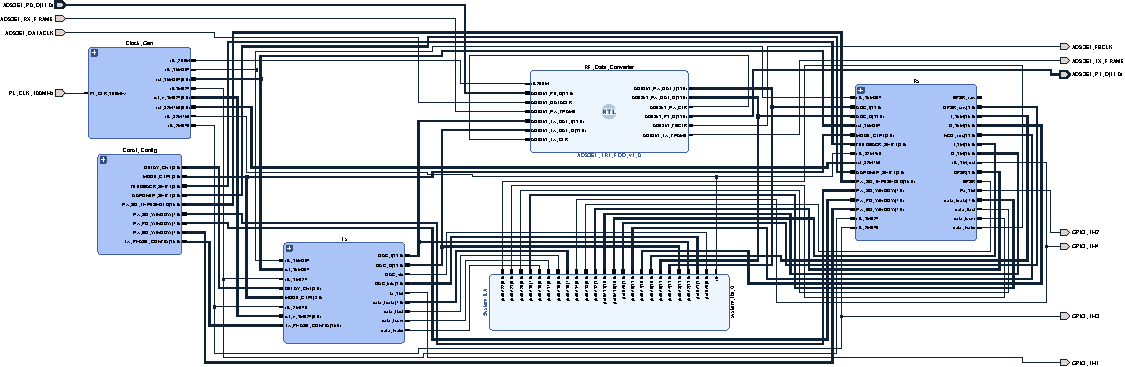
\includegraphics[width=\linewidth]{../schematic/top.pdf}
        \caption{Top block diagram.}
      \end{figure*}

    \subsection{Debugging With Block Diagrams}

      \textbf{AXI connections}.
      1. connection one out of the bus.
      2. \texttt{FREQ\_HZ} property.

      \textbf{Testbenches for block diagrams}.


  \section{Figures in This Paper}

    All figures except for block diagrams in this paper
    are created using T\textit{i}kZ, part of \LaTeX{}.
    The way I create them is quite interesting,
    and you can find the source code in the GitHub repository \cite{github_repo}.

  \bibliographystyle{IEEEtran}
  \bibliography{IEEEabrv, ref}

\end{document}
